\documentclass[12pt]{article}
\usepackage[utf8]{inputenc}
\usepackage[T1]{fontenc}
\usepackage{graphicx}
\usepackage{xcolor}

\usepackage{tikz}
\usepackage{calc}
\usepackage{booktabs}
%\usepackage{hyperref}

% colors
\definecolor{color1}{HTML}{000060}
\definecolor{color2}{HTML}{333333}



% fonts
\usepackage{fontspec}
\defaultfontfeatures{Mapping=tex-text}
\setmainfont
[BoldFont=Lato-Bold.ttf,
ItalicFont=Lato-Italic.ttf,
BoldItalicFont=Lato-BoldItalic.ttf]
{Lato-Regular.ttf}
\newfontfamily\headingfont[ItalicFont=Lato-BlackItalic.ttf]{Lato-Black.ttf}
%%%

\usepackage{geometry}
\geometry{a4paper,
hmargin=20mm,vmargin=20mm,
head=0ex,foot=3ex}

\linespread{1.3}

\usepackage[hang]{caption}
\DeclareCaptionFormat{upper}{#1#2\uppercase{#3}\par}
\captionsetup{labelfont={bf,color=color2},textfont={normalsize,color=color2},format = upper,figurename=FIGURE,tablename=TABLE}

%%% fancy sections
\usepackage{titlesec}
%\titleformat{\chapter}{\headingfont\LARGE\bfseries\scshape\color{color1}}{\thechapter}{1em}{}[\titlerule]
\titleformat{\section}{\color{color1}\headingfont\Large\bfseries\uppercase}{\thesection}{1em}{}[\titlerule]
\titleformat{\subsection}{\color{color1}\headingfont\large\bfseries\uppercase}{\thesubsection}{1em}{}
\titleformat{\subsubsection}{\color{color1}\headingfont\bfseries\uppercase}{\thesubsubsection}{1em}{}
%%%

% head and foot
\usepackage{fancyhdr}
\pagestyle{fancy}
\lhead{}
\chead{}
\makeatletter
\rhead{\color{color2}\@date}
\makeatother
\newlength{\myheight}
\lfoot{
\settoheight{\myheight}{\thepage}
\raisebox{-2ex-0.5\myheight}{
\includegraphics[height=4ex]{logo}}
}
\cfoot{\color{color2}Dr. Scratch: guía docente}
\rfoot{\color{color2}\thepage}
\renewcommand\headrulewidth{0pt}
\renewcommand\footrulewidth{0pt}

%%% picture on cover page
\usepackage{eso-pic}
\newcommand\BackgroundPic{%
\put(0,0){%
\parbox[b][\paperheight]{\paperwidth}{%
\vfill
\centering

\includegraphics[width=\paperwidth,height=\paperheight,%
keepaspectratio]{cover}%
\vfill
}}}
%%%
% custom titlepage
\makeatletter
\renewcommand{\maketitle}{
\thispagestyle{empty}
\AddToShipoutPicture*{\BackgroundPic}
\ClearShipoutPicture
%
\phantom{a}
%\vfill
\vspace{8cm}
\phantom{a}\hfill
\begin{tabular}[c]{@{}p{0.7\textwidth}@{}}
      \color{black}\headingfont\LARGE\@title\\[1em]
      \color{black}\headingfont\Large\@author\\[2em]
\end{tabular}
%
\clearpage
}
\makeatother
%%%


%%% fancy boxes
\usepackage{tcolorbox}
\usepackage{wrapfig}
\def\fullboxbegin{
\bigskip
\begin{tcolorbox}[colback=color1,colframe=color1,coltext=white,arc=0mm,boxrule=0pt]
}
\def\fullboxend{\end{tcolorbox}\medskip}
%
\def\leftboxbegin{
\begin{wrapfigure}{l}{0.5\textwidth}
\begin{tcolorbox}[colback=color1,colframe=color1,coltext=white,arc=0mm,boxrule=0pt]
}
\def\leftboxend{
\end{tcolorbox}
\end{wrapfigure}
}
%
\def\rightboxbegin{
\begin{wrapfigure}{r}{0.5\textwidth}
\begin{tcolorbox}[colback=color1,colframe=color1,coltext=white,arc=0mm,boxrule=0pt]
}
\def\rightboxend{
\end{tcolorbox}
\end{wrapfigure}
}
%
\newcounter{frames}
\def\frameboxbegin#1{
\bigskip
\refstepcounter{frames}
\begin{tcolorbox}[colback=white,colframe=color1,arc=0mm,title={\MakeUppercase{#1}}]
}
\def\frameboxend{
\end{tcolorbox}
}
%%%

\usepackage{lipsum}
\usepackage[spanish]{babel}

%%%%%%%%%%%%%%%
% Title Page
\title{G\'iua docente:  uso de Dr.  Scratch para el desarrollo del pensamiento computacional}
\author{Gregorio Robles, Jes\'us Moreno, Mar\'ia Luz Aguado, Eva Hu}
\date{\today}
%%%%%%%%%%%%%%%

\begin{document}
\maketitle

\tableofcontents
\clearpage

\section*{Licencia}
FIXME: texto de la licencia con la que compartimos el documento.

\section{Introducci\'on}

En los \'ultimos a\~nos estamos presenciando un movimiento global que defiende que el pensamiento computacional deber\'ia ser incluido en la formaci\'on de todos los ni\~nos y ni\~nas, ya que no solo representa un ingrediente vital del aprendizaje de la ciencia, la tecnolog\'ia, la ingenier\'ia y las matem\'aticas, sino que es una competencia fundamental para una vida plena en la sociedad digital hacia la que nos dirigimos.

\subsection*{Pero, �qu\'e es el pensamiento computacional?}
Jeannette Wing, en su art\'iculo \textit{Computational Thinking}\footnote{https://www.cs.cmu.edu/~CompThink/papers/Wing06.pdf} establece que el ``pensamiento computacional implica resolver problemas, dise\~nar sistemas y comprender el comportamiento humano, haciendo uso de los conceptos fundamentales de la inform\'atica''. Es decir, que la esencia del pensamiento computacional es pensar como lo har\'ia un inform\'atico cuando nos enfrentamos a un problema, de manera que podamos aprovechar la potencia de los ordenadores para resolverlos.

Otras definiciones de pensamiento computacional han ido surgiendo en la literatura cient\'ifica desde entonces. Entre las m\'as aceptadas se encuentran la de Aho\footnote{http://comjnl.oxfordjournals.org/content/55/7/832.abstract} y la de la Royal Society\footnote{https://royalsociety.org/education/policy/computing-in-schools/report/}:
\begin{itemize}
 \item El pensamiento computacional es el proceso que permite formular problemas de forma que sus soluciones pueden ser representadas como secuencias de instrucciones y algoritmos.
 \item El pensamiento computacional es el proceso de reconocimiento de aspectos de la inform\'atica en el mundo que nos rodea, y aplicar herramientas y t\'ecnicas de la inform\'atica para comprender y razonar sobre los sistemas y procesos tanto naturales como artificiales.
\end{itemize}

Una iniciativa muy interesante en relaci\'on a la definici\'on del pensamiento computacional es la promovida por la Sociedad Internacional de la Tecnolog\'ia en la Educaci\'on (ISTE) y la Asociaci\'on de Profesores de Inform\'atica (CSTA), que han colaborado con l\'ideres del mundo de la investigaci\'on y la educaci\'on superior, la industria y la educaci\'on primaria y secundaria para desarrollar una definici\'on operativa\footnote{http://csta.acm.org/Curriculum/sub/CurrFiles/CompThinkingFlyer.pdf} que describa con precisi\'on sus caracter\'isticas esenciales y ofrezca un marco de trabajo y un vocabulario com\'un con el que los profesionales de la educaci\'on puedan trabajar.

Seg\'un esta definici\'on operativa, el pensamiento computacional es un proceso de resoluci\'on de problemas que incluye las siguientes caracter\'isticas:

\begin{itemize}
 \item Formular problemas de forma que se permita el uso de un ordenador y otras herramientas para ayudar a resolverlos.
 \item Organizar y analizar l\'ogicamente la informaci\'on.
 \item Representar la informaci\'on a trav\'es de abstracciones como los modelos y las simulaciones.
 \item Automatizar soluciones haciendo uso del pensamiento algor\'itmico (estableciendo una serie de pasos ordenados para llegar a la soluci\'on).
 \item Identificar, analizar e implementar posibles soluciones con el objetivo de lograr la combinaci\'on m\'as efectiva y eficiente de pasos y recursos.
 \item Generalizar y transferir este proceso de resoluci\'on de problemas para ser capaz de resolver una gran variedad de familias de problemas.
\end{itemize}

\subsection*{Programaci\'on inform\'atica y pensamiento computacional}
Aunque el pensamiento computacional puede trabajarse desde muchas disciplinas e incluso sin necesidad de contar con dispositivos electr\'onicos, diversas investigaciones demuestran que la programaci\'on inform\'atica es una muy buena herramienta para desarrollar esta competencia. (FIXME referencia)

Por consiguiente, responsables educativos de todo el mundo han comenzado a incluir la programaci\'on en los curriculum nacionales y regionales. Los ejemplos con mayor repercusi\'on han sido, en el panorama internacional, los de Inglaterra, con una nueva asignatura ``Computing'' obligatoria desde primero de primaria, y Estonia, donde la programaci\'on se usa de manera transversal para trabajar diversas asignaturas de primaria y secundaria; y en el caso de Espa\~na, los de Navarra, que ha incluido la programaci\'on en 4� y 5� de primaria asociada al \'area de matem\'aticas, y la Comunidad de Madrid, que ha incluido contenidos de programaci\'on en la asignatura de tecnolog\'ia de secundaria y ha creado una asignatura optativa de programaci\'on en primaria.

Desde la propia Comisi\'on Europea se est\'a urgiendo a los ministros de la Uni\'on a incluir la programaci\'on inform\'atica en los planes de estudio para que todos los ni\~nos y ni\~nas tengan la oportunidad de desarrollar su pensamiento computacional desde la escuela, ya que estan convencidos de la importancia de esta competencia para la competitividad y la innovaci\'on de nuestro continente. (FIXME referencia)En consecuencia, en los pr\'oximos a\~nos veremos c\'omo la programaci\'on se incluye de forma paulatina en los curriculum de todos los p\'aises europeos, muy probablemente desde la educaci\'on primaria.

\subsection*{C\'omo trabajar y evaluar el pensamiento computacional}
Sin duda alguna, la inclusi\'on de actividades de programaci\'on con \texttt{Scratch}, un lenguaje de programaci\'on visual desarrollado espec\'ificamente para ni\~nos a partir de 6 a\~nos, se est\'a implantando en todo el mundo como el est\'andar para introducir la programaci\'on y trabajar el pensamiento computacional en la educaci\'on. De hecho, en el momento de escribir este texto, hay m\'as de 8 millones de usuarios registrados en la web de \texttt{Scratch} y m\'as de 11 millones de proyectos compartidos.

No obstante, aunque es posible encontrar r\'ubricas preparadas por distintas entidades educativas para evaluar el pensamiento computacional del alumnado a partir de los proyectos \texttt{Scratch} desarrollados por los aprendices, no existen apenas herramientas que permitan automatizar parte de este proceso para ayudar a los docentes. En consecuencia, muchos docentes tienen problemas para poder estudiar en profundidad los proyectos de sus alumnos y poder sacar conclusiones para, por ejemplo, aconsejar a sus alumnos acerca de otros bloques que podr\'ian incorporar a sus programas, formar grupos de estudiantes para trabajar un concepto espec\'ifico que no parecen haber comprendido completamente, o plantearles proyectos avanzados para desarrollar un aspecto concreto una vez alcanzado un determinado nivel. Y este es el motivo que nos llev\'o a crear la herramienta \texttt{Dr.}{\tiny{ }}\texttt{Scratch}, con el objetivo fundamental de asistir a los docentes en el proceso de ense\~nanza y evaluaci\'on de esta competencia.

\subsection*{Dr. Scratch y el pensamiento computacional}
La herramienta \texttt{Dr.}{\tiny{ }}\texttt{Scratch} permite, entre otras funcionalidades, evaluar el grado de desarrollo del pensamiento computacional a partir de un programa \texttt{Scratch}. Las dimensiones evaluadas son las siguientes:
\begin{itemize}
 \item Abstracci\'on y descomposici\'on de problemas
 \item Nociones de algoritmia y control del flujo de los programas
 \item Pensamiento l\'ogico
 \item Paralelismo
 \item Sincronizaci\'on
 \item Representaci\'on de la informaci\'on
 \item Interactividad con el usuario
\end{itemize}
\section{Usando Dr.  Scratch}
FIXME: quiz�s aqu� podr�amos meter un par de capturas explicando c�mo se analizan proyectos con Dr. Scratch.
\section{Desarrollando los distintos aspectos del pensamiento computacional con Dr.  Scratch}
Para cada una de las dimensiones del pensamiento computacional que \texttt{Dr.}{\tiny{ }}\texttt{Scratch} eval\'ua, la herramienta asigna una puntuaci\'on entre 0 y 3 puntos, en funci\'on del grado de desarrollo demostrado en la programaci\'on del proyecto analizado. Para aquellas dimensiones en las que existe margen de mejora, \texttt{Dr.}{\tiny{ }}\texttt{Scratch} ofrece informaci\'on para conocer nuevas posibilidades y seguir mejorando cada uno de estos aspectos.
\subsection{Abstracci\'on y descomposici\'on de problemas}
La capacidad de abstracci\'on y descomposici\'on de problemas te ayuda a dividir un problema en partes m\'as peque\~nas que ser\'an m\'as f\'aciles de comprender, programar y depurar.

\subsubsection{Si has sacado 0 puntos...}
Cuando se comienza a programar con \texttt{Scratch}, en ocasiones puede parecer que la soluci\'on m\'as sencilla es programar todo el comportamiento de un personaje en un \'unico programa. Sin embargo, lo ideal es que el comportamiento del personaje sea controlado por diferentes programas y que cada uno de estos programas se ocupe de una cuesti\'on concreta. Veamos un ejemplo:

\begin{figure}[!h]
\centering
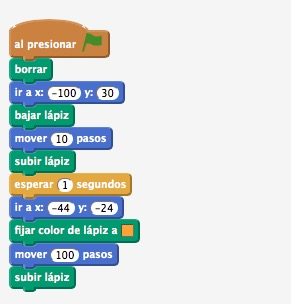
\includegraphics[width=0.25\textwidth]{img/abs1.jpg}
\caption*{Figura 1: Fragmento de c\'odigo con nivel 0 en abstracci\'on.}
\end{figure}


Este proyecto, que pinta un dibujo en la pantalla, ha sido programado en un \'unico programa que dibuja las dos l\'ineas que componen el dibujo. Aunque es una opci\'on v\'alida, una opci\'on m\'as sencilla de programar y de mantener es dividir el programa en dos partes, de forma que tengamos dos programas diferentes, uno para pintar la primera l\'inea y otro para pintar la segunda:
\newpage

\begin{figure}[!h]
\centering
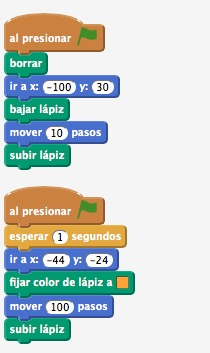
\includegraphics[width=0.25\textwidth]{img/abs2.jpg}
\caption*{Figura 2: Fragmento de c\'odigo con nivel 1 en abstracci\'on.}
\end{figure}


De este modo, si queremos por ejemplo realizar alguna modificaci\'on en una de las l\'ineas dibujadas, es mucho m\'as sencillo saber a qu\'e parte del programa tenemos que dirigirnos para llevar a cabo los cambios.
\subsubsection{Si has sacado 1 punto...}
\texttt{Scratch} permite crear nuevos bloques definidos por los usuarios que se componen de una secuencia de instrucciones. Estas abstracciones permiten crear programas m\'as sencillos de leer, de programar y de mantener. Veamos un ejemplo: 

\begin{figure}[!h]
\centering
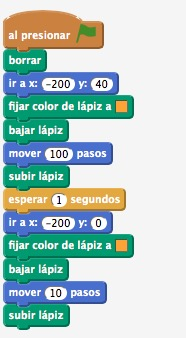
\includegraphics[width=0.25\textwidth]{img/abs3.jpg}
\caption*{Figura 3: Fragmento de c\'odigo con bloques repetidos.}
\end{figure}


Este proyecto \texttt{Scratch}  dibuja dos l\'ineas naranjas de diferente longitud en la pantalla. En lugar de repetir el c\'odigo 2 veces, tal como vemos en el ejemplo, es posible definir un bloque ?PintaNaranja? que se compone de los bloques que pintan una l\'inea naranja en la pantalla y al que se le puede indicar cu\'al es la longitud de la l\'inea. Para ello hay que irse a la categor\'ia ?M\'as Bloques? y pulsar en el bot\'on Crear un bloque:

\begin{figure}[!h]
\centering
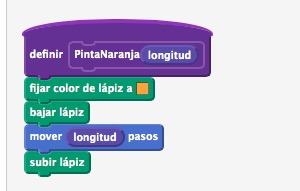
\includegraphics[width=0.25\textwidth]{img/abs4.jpg}
\caption*{Figura 4: Funci\'on propia para evitar repetir c\'odigo.}
\end{figure}


Una vez definido el bloque ?PintaNaranja? es posible utilizarlo en cualquier programa del proyecto, tal como vemos a continuaci\'on:

\begin{figure}[!h]
\centering
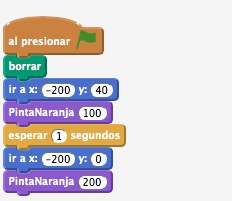
\includegraphics[width=0.25\textwidth]{img/abs5.jpg}
\caption*{Figura 5: Usando nuestra propia funci\'on.}
\end{figure}


De este modo, evitamos la repetici\'on de c\'odigo, lo que hace que nuestros proyectos sean m\'as f\'aciles de programar y mantener. Tal como se puede observar, la primera vez que se usa el bloque PintaNaranja se le indica una longitud de 100 pasos, mientras que la segunda vez la longitud es de 200 pasos.
\subsubsection{Si has sacado 2 puntos...}

En algunos proyectos \texttt{Scratch} queremos tener muchos personajes iguales que realizan exactamente las mismas acciones. La primera idea que se nos ocurre para conseguirlo es crear un personaje, programar todo su comportamiento y, una vez que est\'a listo, crear tantas copias como necesitemos. Por tanto, si queremos 20 marcianitos, hay que crear 20 objetos iguales. Sin embargo, �qu\'e ocurrir\'ia si quiero realizar un cambio en un programa? Tendr\'ia que ir objeto por objeto realizando esa modificaci\'on.

Para este tipo de situaciones es preferible utilizar clones, un tipo de abstracci\'on que nos ayuda a poder programar un solo objeto, y crear de forma din\'amica copias exactas con el mismo comportamiento. 
Veamos c\'omo funcionan con un ejemplo. Imagina que queremos simular que est\'a nevando en un proyecto. Podemos dibujar un objeto que sea un copo de nieve, y una vez que comience la ejecuci\'on del proyecto, ir creando clones constantemente que aparezcan en la parte superior de la pantalla y vayan cayendo hasta la parte inferior:

\begin{figure}[!h]
\centering
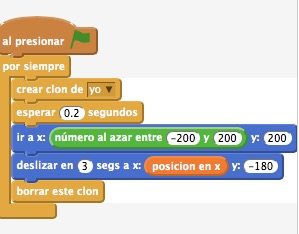
\includegraphics[width=0.25\textwidth]{img/abs6.jpg}
\caption*{Figura 6: Usando clones.}
\end{figure}


De este modo, tan solo programando un personaje podemos tener infinitos clones, que se crean en un momento determinado de la ejecuci\'on del proyecto y se borran cuando ya no son necesarios.

\fullboxbegin
En resumen...
Aprender a abstraer ayuda a ver grandes problemas dif\'iciles de resolver en peque\~nos problemas de f\'acil soluci\'on, favoreciendo, adem\'as, a que se desarrolle un proyecto de una forma m\'as eficiente.
\fullboxend

\frameboxbegin{Ejercicio}
Vamos a proponer un ejercicio para practicar la abstracci\'on. Construye un programa en Scratch en el que el personaje tenga que pintar las letras A, B y C.
\frameboxend

\subsection{Nociones de algoritmia y control del flujo de los programas}
Las instrucciones relacionadas con las nociones algor\'itmicas de control de flujo pueden ayudarte a controlar el comportamiento de tus personajes, haciendo, por ejemplo, que repitan ciertos bloques un n\'umero de veces concreto o que lo repitan hasta que se produzca una situaci\'on.
\subsubsection{Si has sacado 0 puntos...}
La forma m\'as b\'asica de controlar el comportamiento de tus personajes es creando un programa compuesto por un conjunto de bloques que se ejecutan uno detr\'as de otro, tal como vemos en la imagen:

\begin{figure}[!h]
\centering
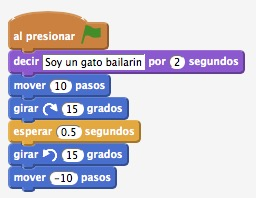
\includegraphics[width=0.25\textwidth]{img/flow1.jpg}
\caption*{Figura 7: Fragmento de c\'odigo con un solo flujo.}
\end{figure}

\newpage
�C\'omo funciona este programa? Cuando el usuario presione sobre la bandera verde se ejecutar\'an uno detras de otro todos los bloques que se han incluido en el programa. Comenzar\'a por el primero 'decir soy un gato que baila por 2 segundos', luego ejecutar\'a 'mover 10 pasos', a continuaci\'on 'girar 15 grados a la derecha', y as\'i hasta llegar al \'ultimo bloque del programa.

\subsubsection{Si has sacado 1 punto...}
En ocasiones, cuando queremos que un conjunto de bloques se repita constantemente, en lugar de repetir los mismos bloques una y otra vez, es posible utilizar instrucciones de repetici\'on que permiten conseguir el mismo efecto, pero de forma m\'as c\'omoda y manejable. Veamos un par de ejemplos:

\begin{figure}[!h]
\centering
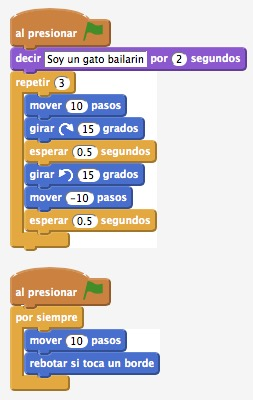
\includegraphics[width=0.25\textwidth]{img/flow2.jpg}
\caption*{Figura 8: Fragmentos de c\'odigo con dos flujos de ejecuci\'on.}
\end{figure}

�C\'omo funciona estos bloques de control? En el bloque 'repetir', cuando la ejecuci\'on llega a este punto se repetir\'an tantas veces como se haya indicado en el par\'ametro del bloque 'repetir', en el ejemplo ser\'ian 3 veces, todos los bloques incluidos dentro de este bloque. Podemos ver que el bloque 'repetir' tiene una flechita en la parte inferior que indica que cuando se terminan de ejecutar los bloques se vuelve otra vez para arriba. El bloque 'por siempre' funciona igual que el 'repetir' pero sin terminar nunca de ejecutar los bloques que contiene en su interior.

\subsubsection{Si has sacado 2 puntos...}
En algunas ocasiones no sabemos previamente el n\'umero de veces que queremos que un conjunto de bloques se ejecute, ya que esto depende de una determinada situaci\'on. En estas ocasiones, el bloque 'repetir hasta que...' es realmente \'util. Veamos un ejemplo:

\begin{figure}[!h]
\centering
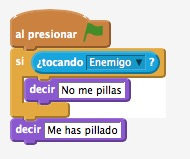
\includegraphics[width=0.25\textwidth]{img/flow3.jpg}
\caption*{Figura 9: Usando el bloque 'si'.}
\end{figure}

En el ejemplo, el personaje repetir\'a constantemente la instrucci\'on decir 'No me pillas...' mientras no est\'e tocando al enemigo. En el momento que se cumpla la condici\'on de la instrucci\'on 'repetir hasta que...', terminar\'a de ejecutarse el bloque contenido en su interior y saltar\'a a la siguiente instrucci\'on, en este caso decir' Me pillaste!'.

\fullboxbegin
En resumen...
Aprender sobre algoritmia y control de flujo nos ayuda a esquematizar y a poner orden en las acciones que se realizan en nuestro programa.
\fullboxend

\frameboxbegin{Ejercicio}
Vamos a proponer un ejercicio para practicar el control de flujo. Construye un programa en Scratch en el que se gu\'ie paso a paso a un cocinero a la hora de realizar la receta de tu plato favorito.
\frameboxend

\subsection{Pensamiento l\'ogico}
Las instrucciones relacionadas con el pensamiento l\'ogico pueden ayudarte a que tus proyectos sean din\'amicos, de forma que se comporten de modo distinto en funci\'on de la situaci\'on. En las historias, por ejemplo, este tipo de instrucciones no son tan importantes, ya que suelen tener una estrucutura lineal que siempre queremos que se ejecute del mismo modo, pero en otro tipo de proyectos, como los videojuegos, son fundamentales para ejecutar acciones diferentes dependiendo de la situaci\'on.
\subsubsection{Si has sacado 0 puntos...}
El bloque m\'as b\'asico con el que puedes comenzar a trabajar el pensamiento l\'ogico es \'este: 

\begin{figure}[!h]
\centering
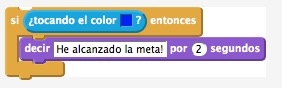
\includegraphics[width=0.25\textwidth]{img/logic1.jpg}
\caption*{Figura 10: Usando el bloque 'si'.}
\end{figure}

�C\'omo funciona este bloque? Cuando la ejecuci\'on llega a este punto, se eval\'ua la condici\'on que aparece en el bloque, y si \'esta es verdadera, se ejecuta el conjunto de bloques que est\'an dentro del si. En el ejemplo, si el personaje est\'a tocando el color azul dir\'ia ?Llegu\'e a la meta?.
\subsubsection{Si has sacado 1 punto...}
Ahora que conoces las instrucciones si, quiz\'as puedas comenzar a utilizar bloques si/sino, que pueden ser muy pr\'acticos en muchos tipos de proyectos. Los bloques si/sino son muy parecidos a los bloque si, pero contienen dos conjuntos de bloques en su interior.

\begin{figure}[!h]
\centering
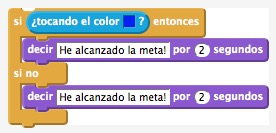
\includegraphics[width=0.25\textwidth]{img/logic2.jpg}
\caption*{Figura 11: Usando el bloque 'si, si no'.}
\end{figure}

�C\'omo funciona este bloque? Cuando la ejecuci\'on llega a este punto, se eval\'ua la condici\'on que aparece en el bloque, y si \'esta es verdadera, se ejecuta el conjunto de bloques que est\'an dentro del si. En el ejemplo, si el personaje est\'a tocando el color azul dir\'ia ?Llegu\'e a la meta?,pero si no est\'a tocando el color morado dir\'ia ?A\'un no he llegado a la meta?.
\subsubsection{Si has sacado 2 puntos...}
Para tomar decisiones en algunos proyectos en ocasiones se requiere evaluar m\'as de una condici\'on al mismo tiempo para saber qu\'e hay que ejecutar. En esas situaciones es muy \'util utilizar operaciones l\'ogicas que permiten combinar las condiciones. Las operaciones l\'ogicas disponibles en Scratch son Y, O y No.

\begin{figure}[!h]
\centering
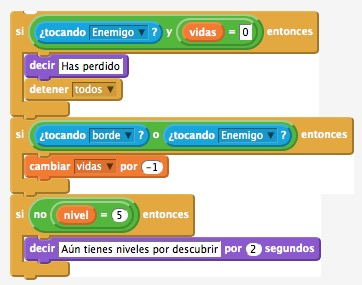
\includegraphics[width=0.25\textwidth]{img/logic3.jpg}
\caption*{Figura 12: Evaluando condiciones.}
\end{figure}

La operaci\'on Y es verdadera cuando las dos condiciones de evaluadas son verdaderas. La operaci\'on O es verdadera cuando una de las dos condiciones evaluadas son verdaderas. Y la operaci\'on No valdr\'a lo contrario de la condici\'on, es decir, si la condici\'on es verdadera, No devuelve falso y viceversa.

\fullboxbegin
En resumen...
El pensamiento l\'ogico nos ayuda a ejecutar cierto c\'odigo si se cumplen unas determinadas condiciones, evitando ejecutarlo cuando no es necesario.
\fullboxend

\frameboxbegin{Ejercicio}
(PENSAR EJERCICIO)
\frameboxend
\subsection{Paralelismo}
En la mayor\'ia de las creaciones Scratch se requiere un cierto nivel de paralelismo. Pero, �qu\'e es el paralelismo? El paralelismo es la posibilidad de que varias cosas ocurran al mismo tiempo. Por ejemplo, que dos personajes realicen una acci\'on al mismo tiempo, o que un personaje haga varias cosas a la vez.
\subsubsection{Si has sacado 0 puntos...}

La forma m\'as b\'asica y m\'as evidente de conseguir paralelismo es tener varios programas que comienzan con ?Al presionar la bandera verde?:
\begin{figure}[!h]
\centering

\includegraphics[width=0.25\textwidth]{img/paral1.jpg}
\caption*{Figura 13: Bloque "al pulsar bandera verde".}
\end{figure}

De este modo, cuando el usuario pinchase sobre la bandera verde, todos los programas que comienzan con este bloque comenzar\'ian a ejecutarse al mismo tiempo, o en paralelo, como tambi\'en puede decirse. Podr\'ias tener varios programas que comiencen con este bloque en un mismo personaje, si quieres que haga varias cosas a la vez, o en programas de diferentes personajes, si quieres que todos comiencen a realizar una acci\'on al comenzar la ejecuci\'on.
\subsubsection{Si has sacado 1 punto...}
Otra forma de conseguir paralelismo en tus programas es haciendo que ocurran varias cosas cuando el usuario presiona una tecla o hace click sobre un objeto. Veamos un par de ejemplos: 

\begin{figure}[!h]
\centering
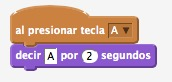
\includegraphics[width=0.25\textwidth]{img/paral2.jpg}
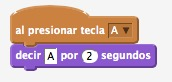
\includegraphics[width=0.25\textwidth]{img/paral2.jpg}
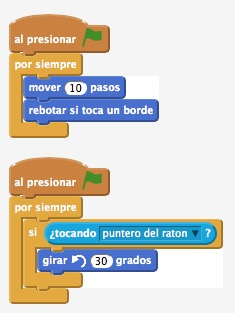
\includegraphics[width=0.25\textwidth]{img/paral3.jpg}
\caption*{Figura 14: C\'odigo que se ejecuta en paralelo.}
\end{figure}

\newpage

�C\'omo funcionan estos bloques de control? En las dos primeras figuras de la izquierda vemos fragmentos de c\'odigo iguales que pertenecen a dos personajes distintos, de manera que, cuando se pulsa una tecla, realizan una determinada acci\'on. Por tanto, cuando el usuario pulse la tecla a, en este caso, tanto un personaje como el otro ejecutar\'an al mismo tiempo ?decir A por 2 segundos?. En el \'ultimo ejemplo vemos que un personaje tiene dos programas que comienzan con ?al clickear este objeto?. Por tanto, cuando el usuario haga click sobre este personaje, ambos programas comenzar\'an a ejecutarse al mismo tiempo, en paralelo.
\subsubsection{Si has sacado 2 puntos...}
Existen varios eventos m\'as que permiten conseguir paralelismo:

\begin{figure}[!h]
\centering
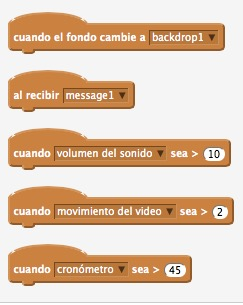
\includegraphics[width=0.25\textwidth]{img/paral4.jpg}
\caption*{Figura 15: Disparadores de eventos.}
\end{figure}

Como ves, podr\'ias crear varios programas que comenzaran a ejecutarse al cambiar el fondo a un determinado escenario, o al recibir un mensaje concreto, o cuando el volumen del ambiente sea superior a un determinado umbral, cuando el movimiento del v\'ideo se mayor que un n\'umero de pixels concreto o cuando el cron\'ometro haya superado el valor que t\'u quieras. Por tanto, existen muchas posibilidades para conseguir que en tus programas ocurran cosas al mismo tiempo. �Te animas a probar algunas de ellas?

\fullboxbegin
En resumen...
El paralelismo nos permite ejecutar varias acciones a la vez en un mismo personaje y/o en varios capturando determinados eventos(teclado, rat\'on, sonido, v\'ideo, mensajes...).
\fullboxend

\frameboxbegin{Ejercicio}
(PENSAR EJERCICIO)
\frameboxend


\subsection{Sincronizaci\'on}
Las instrucciones relacionadas con la sincronizaci\'on permiten organizar a nuestros personajes para que las cosas ocurran en el orden que nosotros deseamos.
\subsubsection{Si has sacado 0 puntos...}
La forma m\'as sencilla de sincronizar el comportamiento de tus personajes es utilizando un bloque 'esperar', que hace que el personaje espere el n\'umero de segundos que escribamos como par\'ametro del bloque. Veamos un ejemplo de c\'omo puede utilizarse este bloque para sincronizar a dos personajes:

\begin{figure}[!h]
\centering
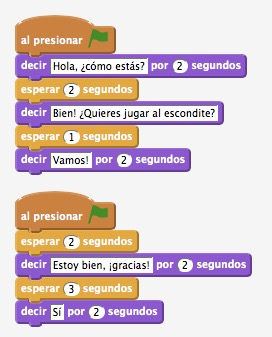
\includegraphics[width=0.25\textwidth]{img/sync1.jpg}
\caption*{Figura 16: Usando bloque es 'esperar'.}
\end{figure}
\newpage
En este caso se han utilizado los bloques esperar' para sincronizar a estos dos personajes para que mantengan una conversaci\'on, de forma que mientras uno habla, el otro espera, y viceversa. F\'ijate en que el n\'umero de segundos que cada personaje espera, son iguales al n\'umero de segundos que el otro personaje habla, de manera que nunca hablan al mismo tiempo.
\subsubsection{Si has sacado 1 punto...}
La sincronizaci\'on mediante bloques 'esperar' es muy sencilla cuando los programas son peque\~nos y tenemos pocos personajes, pero cuando son m\'as grandes, o cuando tenemos varios personajes, o cuando las condiciones para generar una reacci\'on no pueden ser medidas previamente, es m\'as eficiente utilizar otros modos de sincronizaci\'on como los mensajes. Veamos un ejemplo: 
\begin{figure}[!h]
\centering
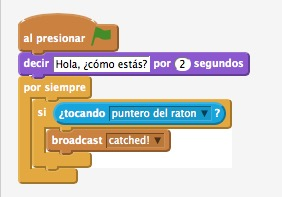
\includegraphics[width=0.25\textwidth]{img/sync2.jpg}
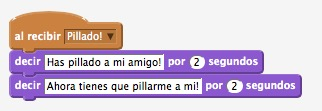
\includegraphics[width=0.25\textwidth]{img/sync3.jpg}
\caption*{Figura 17: Usando env\'io de mensajes.}
\end{figure}

�C\'omo funcionan estos bloques de sincronizaci\'on? Cuando se produce una situaci\'on en un personaje que queremos que provoque una reacci\'on en otro personaje, podemos hacer uso del env\'io de mensajes. En el ejemplo, cuando el rat\'on toca al gato, se env\'ia el mensaje 'Pillado', que ser\'a enviado a todos los personajes del proyecto. As\'i, cuando la mariposa recibe el mensaje 'Pillado', se ejecutan las instrucciones incluidas bajo el bloque 'al recibir Pillado'. Por tanto, cuando el usuario toque con el rat\'on al gato, la mariposa dir\'a: 'Has pillado a mi compa\~nero. Ahora tienes que pillarme a m\'i'.
\subsubsection{Si has sacado 2 puntos...}
Adem\'as del env\'io de mensajes, es posible sincronizar personajes para que las cosas ocurran en el orden que nosotros deseamos utilizando otro tipo de bloques, como 'esperar hasta que' o 'cuando el fondo cambie a...'.

\begin{figure}[!h]
\centering
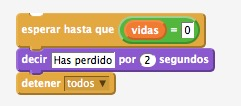
\includegraphics[width=0.25\textwidth]{img/sync4.jpg}
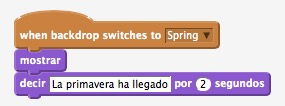
\includegraphics[width=0.25\textwidth]{img/sync5.jpg}
\caption*{Figura 18: Otros bloques de sincronismo.}
\end{figure}

En el primer ejemplo, cuando la ejecuci\'on del programa llegue a ese punto se detendr\'a hasta que se cumpla la condici\'on, en este caso hasta que vidas sea igual a 0. Cuando vidas valga 0, entonces continuar\'a la ejecuci\'on del resto de bloques, en este caso 'decir Game Over' y 'detener todos', lo que finalizar\'a la ejecuci\'on del proyecto. En el segundo ejemplo, en el momento en el que el escenario cambie al fondo con el nombre 'Primavera', el personaje ejecutar\'a los bloques colocados a continuaci\'on de la instrucci\'on 'cuando el fondo cambia a 'Primavera', es decir, que se mostrar\'a y dir\'a '�Ha llegado la primavera'.
\fullboxbegin
En resumen...
El sincronismo permite que las cosas ocurran en el orden que nosotros queramos.
\fullboxend

\frameboxbegin{Ejercicio}
Realizar un programa en Scratch en el que se env\'ie mensajes entre dos personajes.
\frameboxend
\subsection{Representaci\'on de la informaci\'on}
Cada proyecto Scratch necesita un conjunto de informaci\'on sobre los personajes para poder ejecutarse correctamente. Por ejemplo, necesita conocer la posici\'on de cada personaje, la direcci\'on a la que est\'a apuntando, su tama\~no, etc. Adem\'as, los programadores podemos crear nuevos dep\'ositos de informaci\'on para guardar otro tipo de datos, como el nivel en el que nos encontramos, el tiempo transcurrido, la puntaci\'on, las vidas, las recompensas recogidas...
\subsubsection{Si has sacado 0 puntos...}
Cada personaje de un proyecto Scratch tiene una serie de caracter\'isticas, o atributos, que en cada momento de ejecuci\'on del proyecto tienen un valor, y que pueden ser modificadas por los programas. Por ejemplo, un personaje tiene un tama\~no determinado que puede ser modificado por el bloque 'cambiar tama\~no por 10', haciendo que el personaje aparezca un poco m\'as grande. A continuaci\'on mostramos la lista de atributos que tiene cada personaje y los bloques que pueden utilizarse para modificarlos: 
\begin{figure}[!h]
\centering
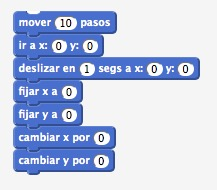
\includegraphics[width=0.25\textwidth]{img/data1.jpg}
\caption*{Figura 19: Posici\'on.}
\end{figure}

\begin{figure}[!h]
\centering
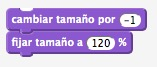
\includegraphics[width=0.25\textwidth]{img/data2.jpg}
\caption*{Figura 20: Tama\~no.}
\end{figure}

\begin{figure}[!h]
\centering
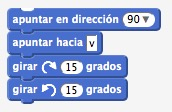
\includegraphics[width=0.25\textwidth]{img/data3.jpg}
\caption*{Figura 21: Orientaci\'on.}
\end{figure}

\begin{figure}[!h]
\centering
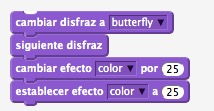
\includegraphics[width=0.25\textwidth]{img/data4.jpg}
\caption*{Figura 22: Disfraz.}
\end{figure}

\begin{figure}[!h]
\centering
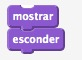
\includegraphics[width=0.25\textwidth]{img/data5.jpg}
\caption*{Figura 23: Visibilidad.}
\end{figure}
\subsubsection{Si has sacado 1 punto...}
Adem\'as de modificar los atributos de los personajes, los programadores podemos utilizar otros mecanismos para almacenar informaci\'on en un proyecto Scratch. Uno de estos mecanismos son las variables, que permiten almacenar un valor para guardar distintos tipos de datos que podemos necesitar: en qu\'e nivel nos encontramos, cu\'antas vidas nos quedan, cu\'antos puntos llevamos, c\'omo se llama el usuario... Para crear una variable hay que irse a la categor\'ia de Datos, pinchar sobre 'Crear una variable' y darle un nombre. En el ejemplo que mostramos a continuaci\'on le hemos dado el nombre 'Puntos', ya que la utilizaremos para guardar el n\'umero de puntos que consigue nuestro personaje. 
\newpage
\begin{figure}[!h]
\centering
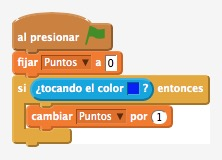
\includegraphics[width=0.25\textwidth]{img/data6.jpg}
\caption*{Figura 24: Variables.}
\end{figure}
En el prorgrama de la izquierda asignamos el n\'umero de puntos con los que queremos que el personaje comience la partida, en este caso 0, para lo que utilizamos el bloque 'fijar Puntos a 0'. Sin embargo en el programa de la derecha lo que hacemos es que cuando el personaje toque el color azul, que podr\'ia ser el de un objetivo, le vamos a sumar un punto, para lo que utilizamos el bloque 'cambiar Puntos por 1'. En este caso, el bloque 'cambiar' comprobar\'ia el valor actual de la variable Puntos y le sumar\'ia 1: si vale 0, le sumo 1 y ahora vale 1; si vale 1, le sumo 1 y ahora vale 2...
\subsubsection{Si has sacado 2 puntos...}
Adem\'as de las variables, Scratch permite utilizar otro tipo de datos para guardar informaci\'on de un proyecto: las listas. Las listas permiten almacenar m\'as de un valor al mismo tiempo, por lo que son ideales para guardar las recompensas que han sido recuperadas por un personaje, o un conjunto de nombres, por plantear un par de ejemplos. Para crear una lista, hay que irse a la categor\'ia de Datos, pinchar sobre 'Crear una lista' y darle un nombre. En el ejemplo, nosotros hemos llamado a nuestra lista 'Estudiantes': 
\begin{figure}[!h]
\centering
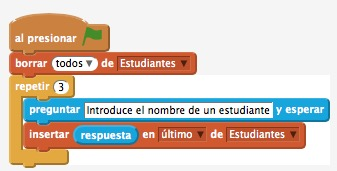
\includegraphics[width=0.5\textwidth]{img/data7.jpg}
\caption*{Figura 25: Otros bloques de sincronismo.}
\end{figure}
\newpage
�Qu\'e hemos hecho con este programa? Lo primero que hacemos al comenzar la ejecuci\'on es borrar todos los elementos de la lista Estudiantes, para vaciarla completamente y que no aparezcan elementos de una ejecuci\'on anterior del proyecto. A continuaci\'on le pedimos tres veces al usuario que introduzca un nombre, y cada nombre introducido lo insertamos en la \'ultima posici\'on de la lista Estudiantes. �Qu\'e podemos hacer con la lista? Podr\'iamos, por ejemplo, utilizarla para sacar a un voluntario a realizar un ejercicio a la pizarra digital. Fijaos en las nuevas instrucciones que a\~nadimos al programa:
\begin{figure}[!h]
\centering
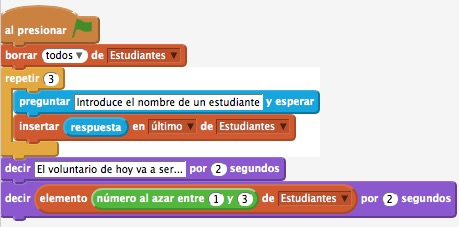
\includegraphics[width=0.5\textwidth]{img/data8.jpg}
\caption*{Figura 26: Otros bloques de sincronismo.}
\end{figure}

Hemos generado un n\'umero al azar entre 1 y 3, que son los elementos que hay en la lista, y hemos seleccionado al elemento que ocupa esa posici\'on en la lista. Unas veces cogeremos el nombre que est\'a en la posici\'on 1, otras al que est\'a en la posici\'on 2 y otras al de la posici\'on 3. Las listas tienen muchas posibilidades y muchas operaciones disponibles... �te animas a investigar c\'omo funcionan?
\fullboxbegin
En resumen...
El sincronismo permite que las cosas ocurran en el orden que nosotros queramos.
\fullboxend

\frameboxbegin{Ejercicio}
Realizar un programa en Scratch en el que se env\'ie mensajes entre dos personajes.
\frameboxend

\subsection{Interactividad con el usuario}

\section{Promoviendo buenos h\'abitos de programaci\'on con Dr.  Scratch}
\subsection{Nombrado de objetos}
\subsection{C\'odigo muerto}
\subsection{Inicializaci\'on de los atributos de los personajes}
\subsection{Repetici\'on de c\'odigo}
\section{Conclusiones finales}
Este documento presenta una gu�a sobre el uso de Dr. Scratch como herramienta de apoyo para desarrollar el pensamiento computacional, que ha sido dise�ada con el objetivo de ayudar a los docentes a comprender las diferentes dimensiones que componen esta competencia, y ofrecer ideas y estrategias para su trabajo en el aula con el alumnado.

Esta gu�a, como todo el proyecto Dr. Scratch, se comparte con una licencia libre y se encuentra disponible en un repositorio p�blico\footnote{https://github.com/kgblll/Documentation/tree/master/LibroDocentes}, de manera que animamos al lector a compartir sus opiniones y cr�ticas para que podamos seguir mejorando el documento, y del mismo modo, le animamos a participar activamente en el desarrollo de la pr�xima versi�n del mismo.
\appendix
\section{Soluci�n a los ejercicios propuestos}
FIXME: Quiz�s podr�an crearse estudios por cada uno de los ejercicios propuestos (que en principio solo tendr�an un proyecto programado por nosotros con la soluci�n), de forma que animemos a la gente a compartir sus soluciones a�adiendo sus proyectos al estudio.

\end{document}          
